\section{Model}
In this section we describe the model that is used to find the speed that will let a vehicle arraive at the next traffic light as it turns green.
See Figure~\ref{fig:Introduction:network} for references.

\subsection{Vehicles}
A vehicle, $\veh$, is an entity that moves along a route.
Each vehicle has an identifier, $\vehid$ a maximum speed, $\vehvel$, a constant acceleration, $\vehacc$ and deceleration, $\vehdec$ and a current position, \vehpos. 
The position is either an edge or a connection (See below).
The position is updated as the vehicle moves.
For simplicity we do not consider different drivering behaviours, but operate with two types of vehicles: cars and trucks. See Table \ref{table.vehicleTypes} for their specifications.
\begin{table}
\centering
\begin{tabular}{|l|l|l|}\hline
		& Car 	& Truck \\\hline
Max speed 	& 	& \\\hline
Acceleration 	&	& \\\hline
Deceleration 	&	& \\\hline
\end{tabular}
\caption{Types of vehicles}\label{table.vehicleTypes}
\end{table}

\subsection{Map}
A map is a directed graph, $G = (V, E, C)$ where $V$ is a set of vertices, $E$ is a set of edges representing road segments and $C$ is a set of connections between edges.
An egde represents one direction of a road segment.
Every edge $\edge\in E$ has a starting point $\estart\in V$, an end point $\eend\in V$ and a maximum speed \espeed. 
The lenght of an edge is the euclidean distance between $\estart$ and \eend denoted as \elength.
In Figure~\ref{fig:Introduction:network} we have five egdes: two to the west of traffic light, two the the east and one to the north. %TODO: Good enough?

Edges are connected through connections.
This way, it is for example possible to model that 
An intersection is made up of several connections that connect road segments one can drive to and from.
For example each possible legal pass through the intersection in Figure~\ref{fig:Introduction:network} is a connection as shown in Figure~\ref{fig:Model:Connection} as red arrows. 
A connection, $\con$ is hence unidirectional from one vertex, $\cestart\in V$ to another vertex, $\ceend \in V$, and a connection is made for each lane of the edges.
A connection is also associated a traffic light phase, $\cphase$. 
The example in Figure~\ref{fig:Introduction:network} hence have six connections assuming one cannot make U-turns.

\begin{figure}[h]
\centering
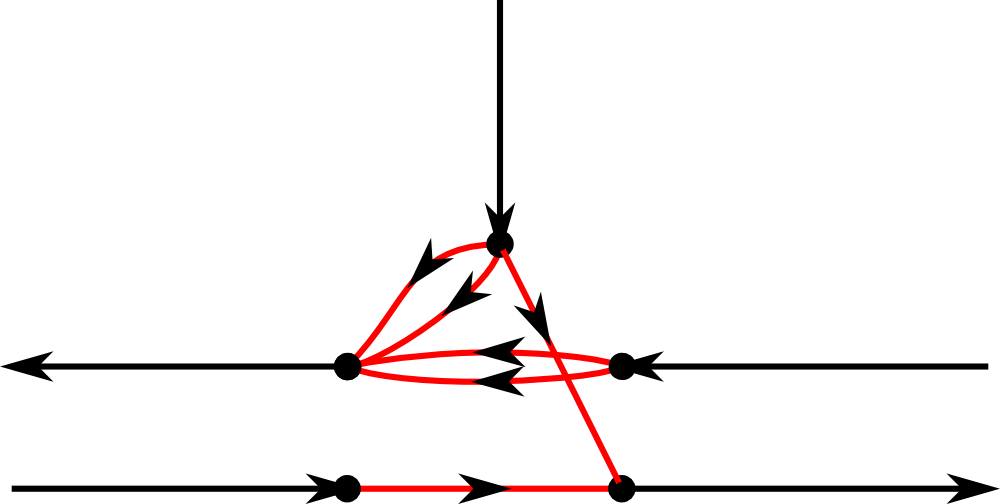
\includegraphics[width=0.4\textwidth]{images/ConnectionNetwork.png}
\caption{Connection network of Figure \ref{fig:Introduction:network}}
\label{fig:Model:Connection}
\end{figure}

\subsection{Sensors}
A sensor can detect whether a vehicle is located at the sensor or not. 
Sensors can for example be induction loops or video cameras. %TODO: More stuff

\subsection{Traffic Light Phases}
We have a traffic light phase for each connection in a traffic light, and each phase details the light setting for just this one connection.
SUMO limits the allowed light settings to $red$, $yellow$ and $green$.
A phase of a traffic light, $\phase$ is defined as $\langle(\light_0, \ti_0),(\light_1, \ti_1),\dots, (\light_n, \ti_n) \rangle$ where the light setting is $\light_i\in \{red, yellow, green\}$ in $\ti_i$ seconds for $0 \leq i \leq n$.
A connection in an unregulated junction will simply have the phase $\langle(green, \infty)\rangle$.
The phases of a traffic light defines the light settings when sensors are not triggered. 


\subsection{Junction}
We define a junction \ju to be a set of connection, $\jucons \subseteq C$. 
A junction can be either regulated or unregulated. 
In an unregulated traffic light normal traffic rules apply. 
In a regulated traffic light vehicles will have to check the phase $\cphase$ of the connection \vehpos. 
A junction is said to be unregulated iff $\forall c \in \jucons | \cphase = \langle(green, \infty)\rangle$

\subsection{Routes}
A route, $\route$, is a sequence of edges on the map, $\langle \edge_0, \edge_1, \dots \edge_n \rangle$, where $\exists \con$ such that $\eendi{i} = \cestart$ and $\estarti{i+1} = \ceend$ for $0\leq i< n$.
The vehicle starts at $\edge_1$ and moves along the sequence until $\edge_n$ has been reached.